\section{More Complex Formulas}
The formulas in the previous section are common formulas, but are fairly simple. The benefit of using temporal logics is that a wide variety of behaviours can be expressed, including propositions about the robot \textit{and} about the workspace. Up to now, we have not looked at any formulas that include atomic propositions about potential tasks. We will show through examples that the same ideas presented in the previous chapter still hold true for this complex tasks, and show the speed up we get by using our algorithm compared to the accepted algorithm. 

\subsection{Example 1}
We look at the example from \cite{guo15} which says "eventually pick up the red ball. Once it is done, move to one basket and drop it. At last come back to room one and stay there". This task can be written as the LTL formula $\varphi = \diamond (\text{rball} \wedge \diamond \text{basket}) \wedge \diamond \square r1$. The B\"uchi automaton corresponding to this formula as translated by \cite{gastin01} is shown in figure \ref{fig:buchiEx1}

\begin{figure}[!htb]
\centering
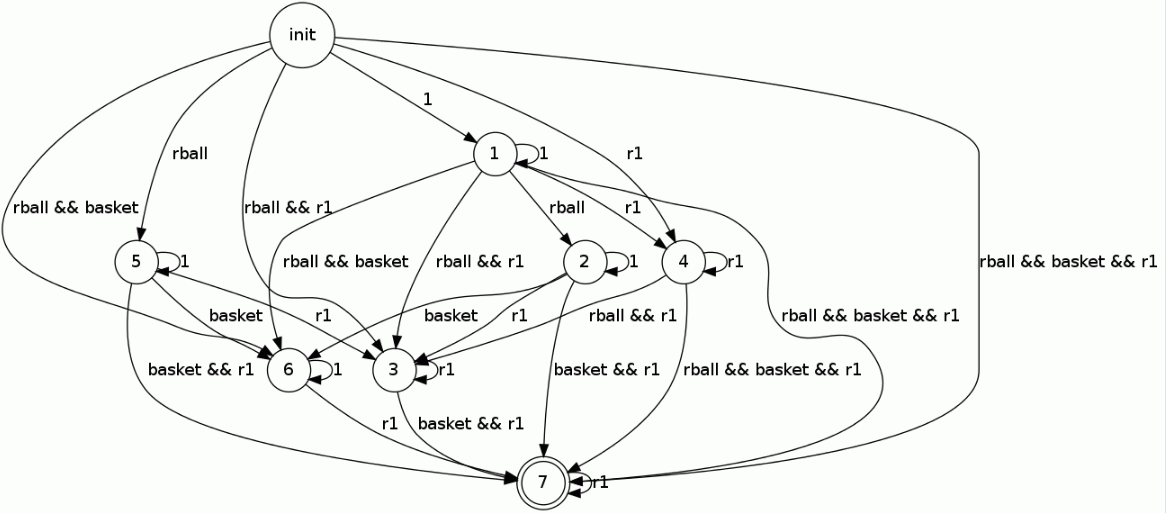
\includegraphics[scale=0.4]{buchiEx1}
\label{fig:buchiEx1}
\end{figure} 

As we can see, there are many edges in this automaton and edges that have \&\& in the label. This paths can only be taken if we satisfy both of the propositions at the same time. However, because in our example the propositions do not overlap (the ball is not in the same room as the basket, and the neither the ball or basket is located in room 1) these edge are impossible to take. Therefore we remove these edges from the automaton (show the code for this). We then have a much simpler automaton that is shown in figure \ref{fig:ex1SimplifiedBuchi}

\begin{figure}
\centering
\begin{tikzpicture}[->,>=stealth',shorten >=1pt,auto,node distance=2.8cm,
                    semithick]
  \tikzstyle{every state}=[fill=red,draw=black,text=black]

  \node[initial,state] (A)                    {$q_1$};
  \node[state] (B)                    [right of=A]{$q_2$};
  \node[state] (C)                    [right of=B]{$q_4$};
  \node[state] (E)                    [above of=B]{$q_3$};
  \node[state] (F)                    [above of=C]{$q_5$};
  \node[state,accepting]         (D) [right of=C] {$q_6$};

  \path (A) edge              node {rball} (B)
  		%(A) edge [loop above] node {$\neg \pi_1$} (A)
  		(B) edge [loop below] node {$\neg$ basket} (B)
  		(B) edge              node {basket} (C)
  		(A) edge              node {$\neg$rball} (E)
  		(E) edge              node {rball} (F)
  		(F) edge              node {basket} (C)
  		(C) edge [loop below] node {$\neg r1$} (C)
  		(C) edge              node {$r1$} (D)
  		(E) edge [loop above] node {$\neg$rball} (E)
  		(F) edge [loop above] node {$\neg$basket} (F)
  		(D) edge [loop above] node {$r1$} (D);
\end{tikzpicture}
\caption{Example 1: $BA$}
\label{fig:ex1SimplifiedBuchi}
\end{figure} 


